% Ubah kalimat sesuai dengan judul dari bab ini
\chapter{TINJAUAN PUSTAKA}

% Ubah konten-konten berikut sesuai dengan yang ingin diisi pada bab ini

\section{Machine Learning}

% Contoh input gambar dengan format *.jpg
% \begin{figure} [ht] \centering
%   % Nama dari file gambar yang diinputkan
%   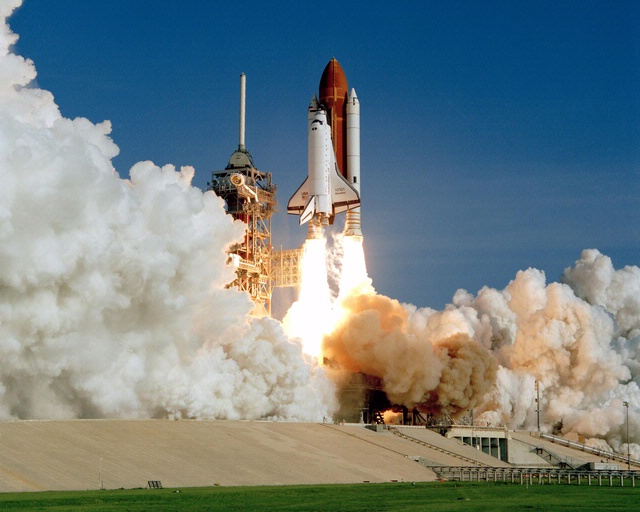
\includegraphics[scale=0.3]{gambar/space-shuttle.jpg}
%   % Keterangan gambar yang diinputkan
%   \caption{Peluncuran pesawat luar angkasa Discovery \citep{DiscoverySpaceShuttle}}
%   % Label referensi dari gambar yang diinputkan
%   \label{fig:SpaceShuttle}
% \end{figure}

Machine Learning (ML) merupakan sebuah cabang dari Artificial Intelligence (kecerdasan buatan) yang memungkinkan sistem
komputer untuk belajar langsung dari contoh, data, dan pengalaman yang didapatkannya. Dengan begitu ML dapat melakukan algoritma kompleks tanpa intruksi / program manual yang dibuat oleh manusia.

Salah satu ciri khas dari ML adalah adanya proses training (pembelajaran). Oleh karena itu, ML membutuhkan data untuk dipelajari yang disebut sebagai data training. Setelah berhasil melakukan
training, maka ML dapat melakukan proses klasifikasi atau prediksi terhadap data baru yang diberikan sesuai dengan hasil training
yang telah dilakukan.

Klasifikasi adalah metode dalam ML yang digunakan oleh mesin untuk memilah atau mengklasifikasikan objek
berdasarkan ciri tertentu sebagaimana manusia mencoba membedakan benda satu dengan yang lain. Sedangkan prediksi digunakan oleh mesin untuk menerka keluaran dari suatu data
masukan. 
% Contoh penggunaan referensi dari gambar yang diinputkan
% \emph{Discovery}, Gambar \ref{fig:SpaceShuttle}, merupakan \lipsum[17][1-9]

\section{Deep Learning}
Deep Learning (DL) adalah salah satu bidang yang muncul dari penelitian ML.
DL memungkinkan model komputasi yang tersusun dari banyak lapisan pemrosesan pembelajaran untuk mempelajari representasi dari data dengan berbagai level.
DL dapat menemukan struktur sulit yang terdapat di dalam kumpulan data yang besar dengan menggunakan algoritma backpropagation.
Struktur yang didapatkan menunjukkan paramater internal apa yang harus diubah oleh mesin agar dapat menghitung representasi di setiap layer berdasarkan representasi dari layer sebelumnya.

DL juga melakukan pendekatan dalam penyelesaian masalah dengan menggunakan konsep hierarki.
Dengan konsep tersebut, komputer mampu mempelajari sebuah konsep yang kompleks dengan menggabungkan
konsep-konsep yang lebih sederhana.

\section{Convolutional Neural Network}
Convolutional Neural Network (CNN) merupakan variasi dari Multilayer Perceptron yang terinspirasi dari jaringan saraf manusia.
Nama convolutional neural network dapat menggambarkan bahwa jaringan ini menggunakan operasi matematika yang disebut konvolusi.
CNN merupakan pengembangan dari artificial neural network yang saat ini diklaim sebagai model terbaik untuk memecahkan masalah
seputar object recognition dan detection.

Secara teknis, CNN adalah arsitektur yang bisa di training
dan terdiri dari beberapa tahap. Input dan output dari masingmasing tahap berupa array yang disebut feature map atau peta
fitur. Output dari masing-masing tahap adalah feature map hasil pengolahan dari semua lokasi pada input. Struktur CNN dibangun
dari tiga jenis layer utama yaitu convolution layer, pooling layer, dan activation function.

\section{Computer Vision}
Computer vision adalah suatu cara menganalisis citra dan video oleh komputer untuk memperoleh hasil sebagaimana yang bisa dilakukan manusia.
Pada hakikatnya, computer vision mencoba meniru cara kerja sistem visual manusia (Human Vision). Manusia melihat objek dengan indra penglihatan (mata),
lalu citra objek diteruskan ke otak untuk diinterpretasi sehingga manusia mengerti objek apa yang tampak dalam pandangan matanya.
Hasil interpretasi ini kemudian digunakan untuk pengambilan keputusan.
Pada komputer, hal ini dilakukan dengan melakukan penangkapan citra atau video melalui kamera, lalu dilakukan proses analisis terhadap gambar tersebut.
Hasil analisis digunakan untuk melakukan keputusan-keputusan yang dibuat berdasarkan kondisi
citra atau video yang ditangkap oleh kamera. Computer vision dibuat agar dapat membantu manusia melakukan proses pengamatan
dan pengambilan keputusan yang sulit jika dilakukan dalam kondisi
yang spesifik.

\section{FaceNet}
FaceNet menggunakan (CNN). CNN ditraining sedemikian rupa sehingga jarak kuadrat L2 antara vector embeddings sesuai dengan kesamaan wajah.
Gambar yang digunakan untuk training telah diskalakan sebelumnya, lalu diubah dan dipotong di sekitar area wajah.
Aspek penting lain dari FaceNet adalah loss functionnya, FaceNet menggunakan triplet loss function dibandingkan model-model lain yang hanya menggunakan single loss function.
Untuk menghitung triplet loss, membutuhkan 3 gambar sebagai acuan yaitu anchor, positif dan negatif.

% \section{Gravitasi}

% Gravitasi merupakan \lipsum[18][1-10]

% \subsection{Hukum Newton}

% % Contoh penggunaan referensi dari pustaka
% Newton \citep{Newton1687} pernah merumuskan bahwa \lipsum[19]
% % Contoh penggunaan referensi dari persamaan
% Kemudian menjadi persamaan seperti pada persamaan \ref{eq:FirstNewtonLaw}.

% % Contoh pembuatan persamaan
% \begin{equation}
%   % Label referensi dari persamaan yang dibuat
%   \label{eq:FirstNewtonLaw}
%   % Baris kode persamaan yang dibuat
%   \sum \mathbf{F} = 0\; \Leftrightarrow\; \frac{\mathrm{d} \mathbf{v} }{\mathrm{d}t} = 0.
% \end{equation}

% \subsection{Anti Gravitasi}

% Anti gravitasi merupakan \lipsum[20]
